% Template for PLoS
% Version 3.5 March 2018
%
% % % % % % % % % % % % % % % % % % % % % %
%
% -- IMPORTANT NOTE
%
% This template contains comments intended
% to minimize problems and delays during our production
% process. Please follow the template instructions
% whenever possible.
%
% % % % % % % % % % % % % % % % % % % % % % %
%
% Once your paper is accepted for publication,
% PLEASE REMOVE ALL TRACKED CHANGES in this file
% and leave only the final text of your manuscript.
% PLOS recommends the use of latexdiff to track changes during review, as this will help to maintain a clean tex file.
% Visit https://www.ctan.org/pkg/latexdiff?lang=en for info or contact us at latex@plos.org.
%
%
% There are no restrictions on package use within the LaTeX files except that
% no packages listed in the template may be deleted.
%
% Please do not include colors or graphics in the text.
%
% The manuscript LaTeX source should be contained within a single file (do not use \input, \externaldocument, or similar commands).
%
% % % % % % % % % % % % % % % % % % % % % % %
%
% -- FIGURES AND TABLES
%
% Please include tables/figure captions directly after the paragraph where they are first cited in the text.
%
% DO NOT INCLUDE GRAPHICS IN YOUR MANUSCRIPT
% - Figures should be uploaded separately from your manuscript file.
% - Figures generated using LaTeX should be extracted and removed from the PDF before submission.
% - Figures containing multiple panels/subfigures must be combined into one image file before submission.
% For figure citations, please use "Fig" instead of "Figure".
% See http://journals.plos.org/plosone/s/figures for PLOS figure guidelines.
%
% Tables should be cell-based and may not contain:
% - spacing/line breaks within cells to alter layout or alignment
% - do not nest tabular environments (no tabular environments within tabular environments)
% - no graphics or colored text (cell background color/shading OK)
% See http://journals.plos.org/plosone/s/tables for table guidelines.
%
% For tables that exceed the width of the text column, use the adjustwidth environment as illustrated in the example table in text below.
%
% % % % % % % % % % % % % % % % % % % % % % % %
%
% -- EQUATIONS, MATH SYMBOLS, SUBSCRIPTS, AND SUPERSCRIPTS
%
% IMPORTANT
% Below are a few tips to help format your equations and other special characters according to our specifications. For more tips to help reduce the possibility of formatting errors during conversion, please see our LaTeX guidelines at http://journals.plos.org/plosone/s/latex
%
% For inline equations, please be sure to include all portions of an equation in the math environment.
%
% Do not include text that is not math in the math environment.
%
% Please add line breaks to long display equations when possible in order to fit size of the column.
%
% For inline equations, please do not include punctuation (commas, etc) within the math environment unless this is part of the equation.
%
% When adding superscript or subscripts outside of brackets/braces, please group using {}.
%
% Do not use \cal for caligraphic font.  Instead, use \mathcal{}
%
% % % % % % % % % % % % % % % % % % % % % % % %
%
% Please contact latex@plos.org with any questions.
%
% % % % % % % % % % % % % % % % % % % % % % % %

\documentclass[10pt,letterpaper]{article}
\usepackage[top=0.85in,left=2.75in,footskip=0.75in]{geometry}

% amsmath and amssymb packages, useful for mathematical formulas and symbols
\usepackage{amsmath,amssymb}

% Use adjustwidth environment to exceed column width (see example table in text)
\usepackage{changepage}

% Use Unicode characters when possible
\usepackage[utf8x]{inputenc}

% textcomp package and marvosym package for additional characters
\usepackage{textcomp,marvosym}

% cite package, to clean up citations in the main text. Do not remove.
% \usepackage{cite}

% Use nameref to cite supporting information files (see Supporting Information section for more info)
\usepackage{nameref,hyperref}

% line numbers
\usepackage[right]{lineno}

% ligatures disabled
\usepackage{microtype}
\DisableLigatures[f]{encoding = *, family = * }

% color can be used to apply background shading to table cells only
\usepackage[table]{xcolor}

% array package and thick rules for tables
\usepackage{array}

% create "+" rule type for thick vertical lines
\newcolumntype{+}{!{\vrule width 2pt}}

% create \thickcline for thick horizontal lines of variable length
\newlength\savedwidth
\newcommand\thickcline[1]{%
  \noalign{\global\savedwidth\arrayrulewidth\global\arrayrulewidth 2pt}%
  \cline{#1}%
  \noalign{\vskip\arrayrulewidth}%
  \noalign{\global\arrayrulewidth\savedwidth}%
}

% \thickhline command for thick horizontal lines that span the table
\newcommand\thickhline{\noalign{\global\savedwidth\arrayrulewidth\global\arrayrulewidth 2pt}%
\hline
\noalign{\global\arrayrulewidth\savedwidth}}


% Remove comment for double spacing
%\usepackage{setspace}
%\doublespacing

% Text layout
\raggedright
\setlength{\parindent}{0.5cm}
\textwidth 5.25in
\textheight 8.75in

% Bold the 'Figure #' in the caption and separate it from the title/caption with a period
% Captions will be left justified
\usepackage[aboveskip=1pt,labelfont=bf,labelsep=period,justification=raggedright,singlelinecheck=off]{caption}
\renewcommand{\figurename}{Fig}

% Use the PLoS provided BiBTeX style
% \bibliographystyle{plos2015}

% Remove brackets from numbering in List of References
\makeatletter
\renewcommand{\@biblabel}[1]{\quad#1.}
\makeatother



% Header and Footer with logo
\usepackage{lastpage,fancyhdr,graphicx}
\usepackage{epstopdf}
%\pagestyle{myheadings}
\pagestyle{fancy}
\fancyhf{}
%\setlength{\headheight}{27.023pt}
%\lhead{
\includegraphics[width=2.0in]{PLOS-submission.eps}}
\rfoot{\thepage/\pageref{LastPage}}
\renewcommand{\headrulewidth}{0pt}
\renewcommand{\footrule}{\hrule height 2pt \vspace{2mm}}
\fancyheadoffset[L]{2.25in}
\fancyfootoffset[L]{2.25in}
\lfoot{\today}

%% Include all macros below

\newcommand{\lorem}{{\bf LOREM}}
\newcommand{\ipsum}{{\bf IPSUM}}



\usepackage{longtable}
\usepackage{booktabs}



\usepackage{forarray}
\usepackage{xstring}
\newcommand{\getIndex}[2]{
  \ForEach{,}{\IfEq{#1}{\thislevelitem}{\number\thislevelcount\ExitForEach}{}}{#2}
}

\setcounter{secnumdepth}{0}

\newcommand{\getAff}[1]{
  \getIndex{#1}{University of Chicago,University at Buffalo, SUNY}
}

\providecommand{\tightlist}{%
  \setlength{\itemsep}{0pt}\setlength{\parskip}{0pt}}

\begin{document}
\vspace*{0.2in}

% Title must be 250 characters or less.
\begin{flushleft}
{\Large
\textbf\newline{Pervasive duplication of tumor suppressor genes preceded parallel
evolution of large bodied Paenungulates} % Please use "sentence case" for title and headings (capitalize only the first word in a title (or heading), the first word in a subtitle (or subheading), and any proper nouns).
}
\newline
% Insert author names, affiliations and corresponding author email (do not include titles, positions, or degrees).
\\
Juan Manuel Vazquez\textsuperscript{\getAff{University of Chicago}}\textsuperscript{*},
Vincent J Lynch\textsuperscript{\getAff{University at Buffalo, SUNY}}\\
\bigskip
\textbf{\getAff{University of Chicago}}Department of Human Genetics, 920 East 58th St, Chicago, IL, 60637\\
\textbf{\getAff{University at Buffalo, SUNY}}Department of Biological Sciences, 551 Cooke Hall, Buffalo NY, 14260\\
\bigskip
* Corresponding author: juanvazquez@uchicago.edu\\
\end{flushleft}
% Please keep the abstract below 300 words
\section*{Abstract}
Lorem ipsum dolor sit amet, consectetur adipiscing elit. Curabitur eget
porta erat. Morbi consectetur est vel gravida pretium. Suspendisse ut
dui eu ante cursus gravida non sed sem. Nullam sapien tellus, commodo id
velit id, eleifend volutpat quam. Phasellus mauris velit, dapibus
finibus elementum vel, pulvinar non tellus. Nunc pellentesque pretium
diam, quis maximus dolor faucibus id. Nunc convallis sodales ante, ut
ullamcorper est egestas vitae. Nam sit amet enim ultrices, ultrices elit
pulvinar, volutpat risus.

% Please keep the Author Summary between 150 and 200 words
% Use first person. PLOS ONE authors please skip this step.
% Author Summary not valid for PLOS ONE submissions.
\section*{Author summary}
Lorem ipsum dolor sit amet, consectetur adipiscing elit. Curabitur eget
porta erat. Morbi consectetur est vel gravida pretium. Suspendisse ut
dui eu ante cursus gravida non sed sem. Nullam sapien tellus, commodo id
velit id, eleifend volutpat quam. Phasellus mauris velit, dapibus
finibus elementum vel, pulvinar non tellus. Nunc pellentesque pretium
diam, quis maximus dolor faucibus id. Nunc convallis sodales ante, ut
ullamcorper est egestas vitae. Nam sit amet enim ultrices, ultrices elit
pulvinar, volutpat risus.

\linenumbers

% Use "Eq" instead of "Equation" for equation citations.
)

\hypertarget{introduction}{%
\section{Introduction}\label{introduction}}

One of the major constraints on the evolution of large body sizes in
animals is an increased risk of developing cancer. If all cells in all
organisms have a similar risk of malignant transformation and equivalent
cancer suppression mechanisms, organism with many cells should have a
higher prevalence of cancer than organisms with fewer cells. Consistent
with this expectation there is a strong positive correlation between
body size and cancer incidence within species, for example, human cancer
incidence increases with increasing adult height {[}1,2{]} and cancer
incidence is positively correlated with body size in dogs
{[}{\textbf{???}},3{]}. There is no correlation, however, between body
size and cancer risk between species. This lack of correlation is often
referred to as `Peto's Paradox' {[}4--6{]}. While it is clear that a
resolution to Peto's Paradox must involve the evolution of enhanced
cancer protection alongside increases in body size and lifespan, the
specific genetic, molecular, and cellular mechanisms that underlie this
resistance have proven elusive. {[}7--11{]}.

Among the challenges for discovering how animals evolved enhanced cancer
protection mechanisms is identifying lineages in which large bodied
species are nested within species with small body sizes. Afrotherian
mammals are generally small-bodied, similarly to the prediced common
ancestor of Eutherian mammals. For example, maximum adult weights are
\textasciitilde{}70g in golden moles, \textasciitilde{}120g in tenrecs,
\textasciitilde{}170g in elephant shrews, \textasciitilde{}3kg in
hyraxes, and 60kg in aardvarks {[}12{]}. However, while these extant
species are relatively small, the fossil evidence demonstrates that
their ancestral lineages reached enormous sizes. For example, while
extant hyraxes are relatively small, the extinct Titanohyrax is
estimated to have weighted up to \textasciitilde{}1300kg {[}13{]}. The
largest members of Afrotheria, too, are dwarfed by the size of their
recent ancestors: extant cows manatees are large bodied
(\textasciitilde{}322-480kg) but are relatively small compared to the
extinct Stellar's sea cow which is estimated to have weight 8000-10000kg
{[}14{]}. Similarly African (4,800kg) and Asian elephants (3,200kg) are
the largest living elephant species, but are dwarfed by the truly
gigantic extinct Proboscideans such as Deinotherium
(\textasciitilde{}132,000kg), Mammut borsoni (110,000kg), and the Asian
straight-tusked elephant (\textasciitilde{}220,000kg), the largest known
land mammal {[}15{]}. Remarkably these large-bodied Afrotherian lineages
are nested within small bodied species (Fig. 1) {[}16--19{]}, indicating
that gigantism independently evolved in hyraxes, sea cows, and elephants
(Paenungulates). Thus, Paenungulates are an excellent model system in
which to explore the mechanisms that underlie the evolution of large
body sizes and augmented cancer resistance.

Although many mechanisms can potentially resolve Peto's paradox, the
most parsimonious route to enhanced cancer resistance is likely through
an increased copy number of tumor suppressors. Such an example has been
seen in the case of candidate genes such as \emph{TP53} and \emph{LIF}
{[}11,20,21{]} as well as in studies involving a limited set of
candidate genes {[}22,23{]}. As these studies focus on \emph{a priori}
gene sets, however, it remains unknown whether this is a general,
genome-wide trend in Afrotherian genomes; and whether such a general
trend is associated with the recent increases in body size -- and
therefore expected cancer risk -- in these species.

Here, we trace the evolution of body mass and gene copy number variation
in Afrotherians in order to investigate whether gene duplications are
enriched in large, long-lived species for genes involved in known tumor
suppression pathways. Our estimates of the evolution of body mass,
similarly to previous studies {[}16--19{]}, show that large body masses
evolved in a step-wise manner, with major increases in body mass in the
Pseudoungulata (17kg), Paenungulata (25kg), Tethytheria (296kg), and
Proboscidea (4,100kg) stem-lineages. Furthermore, we see that the
ancestral body size increases in Hydracoidia and Sirenia were
independent events. To study the evolution of gene copy number, we used
a genome-wide Reciprocal Best BLAT Hit (RBBH) method to identify gene
duplications in Afrotherian genomes, and used parsimony to infer the
lineages in which those duplications occurred. We found gene
duplications in lineages with increased body mass were enriched in
functions related to tumor suppression, including regulation of the cell
cycle, DNA damage repair, and regulation of apoptosis. These data
suggest that duplication of tumor suppressors played a role in the
evolution of large, long-lived in Afrotherians.

\hypertarget{methods}{%
\section{Methods}\label{methods}}

\hypertarget{ancestral-body-size-reconstruction}{%
\subsection{Ancestral Body Size
Reconstruction}\label{ancestral-body-size-reconstruction}}

We built a time-calibrated supertree of Eutherian mammals by combining
the time-calibrated molecular phylogeny of Bininda-Emonds \emph{et al.}
{[}24{]} with the time-calibrated total evidence Afrotherian phylogeny
from Puttick and Thomas {[}{\textbf{???}}{]}. While the Bininda-Emonds
\emph{et al.} {[}24{]} phylogeny includes 1,679 species, only 34 are
Afrotherian, and no fossil data are included. The inclusion of fossil
data from extinct species is essential to ensure that ancestral state
reconstructions of body mass are not biased by only including extant
species. This can lead to inaccurate reconstructions, for example, if
lineages convergently evolved large body masses from a small bodied
ancestor. In contrast, the total evidence Afrotherian phylogeny of
Puttick and Thomas {[}19{]} includes 77 extant species and fossil data
from 39 extinct species. Therefore we replaced the Afrotherian clade in
the Bininda-Emonds \emph{et al.} {[}24{]} phylogeny with the Afrotherian
phylogeny of Puttick and Thomas {[}19{]} using Mesquite. Next, we
jointly estimated rates of body mass evolution and reconstructed
ancestral states using a generalization of the Brownian motion model
that relaxes assumptions of neutrality and gradualism by considering
increments to evolving characters to be drawn from a heavy-tailed stable
distribution (the ``Stable Model'') {[}25{]}. The stable model allows
for occasional large jumps in traits and has previously been shown to
out-perform other models of body mass evolution, including standard
Brownian motion models, Ornstein--Uhlenbeck models, early burst maximum
likelihood models, and heterogeneous multi-rate models {[}25{]}.

\hypertarget{identification-of-duplicate-genes}{%
\subsection{Identification of Duplicate
Genes}\label{identification-of-duplicate-genes}}

\emph{Reciprocal Best-Hit BLAT:} We developed a reciprocal best hit BLAT
(RBHB) pipeline to quickly identify homologs and estimate gene copy
numbers (\textbf{Figure 1A}). The Reciprocal Best Hit (RBH) search
strategy is conceptually straightforward: 1) Given a gene of interest GA
in a query genome A, one searches a target genome B for all possible
matches to GA; 2) For each of these hits, one then performs the
reciprocal search in the original query genome to identify the
highest-scoring hit; 3) A hit in genome B is defined as a homolog of
gene GA if and only if the original gene GA is the top reciprocal search
hit in genome A. We selected BLAT {[}26{]} as our algorithm of choice,
as this algorithm is sensitive to highly simliar (\textgreater{}90\%
identity) sequences, thus identifying the highest-confidence homologs
while minimizing many-to-one mapping problems when searching for
multiple genes. RBH performs similar to other more complex methods of
orthology prediction, and is particularly good at identifying incomplete
genes that may be fragmented in low quality/poor assembled regions of
the genome {[}{\textbf{???}},27{]}.

\emph{Effective Copy Number By Coverage:} In lower-quality genomes, many
genes are fragmented across multiple scaffolds, which results in BLAT
calling multiple hits when in reality there is only one gene. To
compensate for this, we came up with a novel statistic, Estimated Copy
Number by Coverage (ECNC), which averages the number of times we see
each nucleotides of a query sequence in a target genome over the total
number of nucleotides of the query sequence found overall in each target
genome (\textbf{Figure 1B}; Supplementary Figure 1). This allows us to
correct for genes that have been fragmented across incomplete genomes,
without underestimating the copy number of proteins that lack domains
found in the human sequence.

\emph{RecSearch Pipeline:} We created a custom Python pipeline for
automating RBHB searches between a single reference genome and multiple
target genomes using a list of query sequences from the reference
genome. For the query sequences in our search, we used the hg38 Proteome
provided by UniProt {[}28{]}, which is a comprehensive set of protein
sequences curated from a combination of predicted and validated protein
sequences generated by the UniProt Consortium. In order to refine our
search, we omitted protein sequences originating from long, noncoding
RNA loci (e.g.~LINC genes); poorly-studied genes from predicted open
reading frames (C-ORFs); and sequences with highly repetitive sequences
such as zinc fingers, protocadherins, and transposon-containing genes,
as these were prone to high levels of false positive hits. After
filtering out problematic protein queries, we then used our pipeline
(Figure 1A) to search for all copies of our 20456 query genes in
publicly available Afrotherian genomes, including African savannah
elephant (\emph{Loxodonta africana}: loxAfr3, loxAfr4, loxAfrC), African
forest elephant (\emph{Loxodonta cyclotis}: loxCycF), Asian Elephant
(\emph{Elephas maximus}: eleMaxD), Woolly Mammoth (\emph{Mammuthus
primigenius}: mamPriV), Colombian mammoth (\emph{Mammuthus columbi}:
mamColU), American mastodon (\emph{Mammut americanum}: mamAmeI), Rock
Hyrax (\emph{Procavia capensis}: proCap1, proCap2, proCap2\_HiC), West
Indian Manatee (\emph{Trichechus manatus latirostris}: triManLat1,
triManLat1\_HiC), Aardvark (\emph{Orycteropus afer}: oryAfe1,
oryAfe1\_HiC), Lesser Hedgehog Tenrec (\emph{Echinops telfairi}:
echTel2), Nine-banded armadillo (\emph{Dasypus novemcinctus}: dasNov3),
Hoffman's two-toed sloth (\emph{Choloepus hoffmannii}: choHof1, choHof2,
choHof2\_HiC), Cape golden mole (\emph{Chrysochloris asiatica}:
chrAsi1), and Cape elephant shrew (\emph{Elephantulus edwardii}:
eleEdw1). For many of these species, we covered multiple assemblies in
order to test the effects of assembly size and quality on our hits.

\emph{Duplication gene inclusion criteria:} In order to condense
transcript-level hits into single gene loci, and to resolve many-to-one
genome mappings, we removed exons where transcripts from different genes
overlapped, and merged overlapping transcripts of the same gene into a
single gene locus call. The resulting gene-level copy number table was
then combined with the maximum ECNC values observed for each gene in
order to call gene duplications. We called a gene duplicated if its copy
number was two or more, and if the maximum ECNC value of all the gene
transcripts searched was 1.5 or greater; previous studies have shown
that incomplete duplications can encode functional genes, therefore
partial gene duplications were included provided they passed additional
inclusion criteria. The ECNC cut off of 1.5 was selected empirically, as
this value minimized the number of false positives seen in a test set of
genes and genomes. The results of our initial search are summarized in
Figure 1B. Overall, we identified {[}MEDIAN{]} genes across all species,
or {[}\%HITS/QUERIES{]} of our starting query genes. As expected, there
was a correlation between the number of hits identified in a species
with the evolutionary distance relative to humans {[}Sup Figure 1{]}.

\emph{Duplicate gene exclusion criteria:} We excluded genes from
downstream analyses for which assignment of homology was uncertain,
including uncharacterized ORFs (17), LOC (17), HLA genes (17),
replication dependent histones (17), odorant receptors (17), ribosomal
proteins (17), zinc finger transcription factors (17), viral and
repetitive-element-associated proteins (17) and any protein described as
either ``Uncharacterized,'' ``Putative,'' or ``Fragment'' by UniProt in
UP000005640 (17).

\hypertarget{evidence-for-functionality-of-identified-genes}{%
\subsection{Evidence for Functionality of Identified
Genes}\label{evidence-for-functionality-of-identified-genes}}

To validate and filter out RBHB results, we intersected our results with
either gene prediction or transcriptomic evidence as a proxy for
functionality.

\textbf{Transcriptome Assembly:} For the African Savana Elephant, Asian
Elephant, West Indian Manatee, and Nine-Banded Armadillo, we generated
\emph{de novo} transcriptomes using publically-available RNA-sequencing
data from NCBI SRA. We mapped reads to all genomes available for each
species, and assembled transcripts using HISAT2 and StringTie,
respectively {[}{\textbf{???}},{\textbf{??}},{\textbf{??}}{]}.
RNA-sequencing data was not available for Cape Golden Mole, Cape
Elephant Shrew, Rock Hyrax, Aardvark, or the Lesser Hedgehog Tenrec.

\textbf{Gene Prediction:} We obtained tracks for genes predicted using
GenScan for all the genomes available via UCSC Genome Browser: African
savannah elephant (loxAfr3), Rock Hyrax (proCap1), West Indian Manatee
(triManLat1), Aardvark (oryAfe1), Lesser Hedgehog Tenrec (echTel2),
Nine-banded armadillo (dasNov3), Hoffman's Two-Toed Sloth (choHof1),
Cape golden mole (chrAsi1), and Cape Elephant Shrew (eleEdw1); gene
prediction tracks for higher-quality assemblies were not available.

\textbf{Evidenced Duplicate Criteria:} We intersected our records of
duplicate hits identified in each genome with the gene prediction tracks
and/or transcriptome assemblies using \texttt{bedtools}
{[}{\textbf{???}}{]}. When multiple lines of evidence for functionality
were present for a genome, we used the union of all intersections as the
final output for evidenced duplicates. When analyzing the
highest-quality assemblies available for each species, if a species had
neither gene prediction tracks nor RNA-seq data for the highest-quality
genome available, we conservatively included all hits for the genome in
the final set of evidenced duplicates.

\hypertarget{reconstruction-of-ancestral-copy-numbers}{%
\subsection{Reconstruction of Ancestral Copy
Numbers}\label{reconstruction-of-ancestral-copy-numbers}}

We implemented a maximum likelihood method for determining the ancestral
copy numbers of genes in \emph{Atlantogenata} using IQ-Tree. For this
analysis, we used an unrooted subset of our prior species tree,
including only the aforementioned \emph{Atlantogenata} species. We
generated PHYLIP files containing the copy number of each gene in the
highest quality genome for each species, encoding genes on a scale from
1-31+ copies as 1-9, A-V; and encoding a gene's copy number as uncetain
(``?'') when we did not identify it in the genome. We used the included
tree-searching and model-testing functionality in IQ-Tree to determine
the most likely topology for the species tree, and to obtain the most
likely model for copy number changes in the genome. We defined the
ancestral state of a node if it had greater than an 80\% posterior
probability.

\hypertarget{pathway-enrichment-analysis}{%
\subsection{Pathway Enrichment
Analysis}\label{pathway-enrichment-analysis}}

To determine which pathways were associated with duplicated genes in
each species and lineage, we used WEBGESTALT to perform
overrepresentation analysis (ORA) of the duplicated gene lists relative
to our initial query gene list. For the database of pathways used in the
analysis, we used Reactome {[}{\textbf{???}}{]}, Wikipathways and
Wikipathways\_cancer {[}{\textbf{???}}{]}, and KEGG
{[}{\textbf{???}}{]}.

\hypertarget{results}{%
\section{Results}\label{results}}

\begin{verbatim}
## Warning: Tried to calculate with group_by(), but the calculation failed.
## Falling back to ungrouped filter operation...

## Warning: Tried to calculate with group_by(), but the calculation failed.
## Falling back to ungrouped filter operation...
\end{verbatim}

\begin{verbatim}
## Warning in geom2trace.default(dots[[1L]][[3L]], dots[[2L]][[1L]], dots[[3L]][[1L]]): geom_GeomTextRepel() has yet to be implemented in plotly.
##   If you'd like to see this geom implemented,
##   Please open an issue with your example code at
##   https://github.com/ropensci/plotly/issues

## Warning in geom2trace.default(dots[[1L]][[3L]], dots[[2L]][[1L]], dots[[3L]][[1L]]): geom_GeomTextRepel() has yet to be implemented in plotly.
##   If you'd like to see this geom implemented,
##   Please open an issue with your example code at
##   https://github.com/ropensci/plotly/issues

## Warning in geom2trace.default(dots[[1L]][[3L]], dots[[2L]][[1L]], dots[[3L]][[1L]]): geom_GeomTextRepel() has yet to be implemented in plotly.
##   If you'd like to see this geom implemented,
##   Please open an issue with your example code at
##   https://github.com/ropensci/plotly/issues
\end{verbatim}

\hypertarget{step-wise-evolution-of-large-long-lived-afrotherians}{%
\subsection{Step-wise evolution of large, long-lived
Afrotherians}\label{step-wise-evolution-of-large-long-lived-afrotherians}}

\begin{verbatim}
## Warning: Removed 120 rows containing missing values (geom_image).
\end{verbatim}

\begin{longtable}[]{@{}lrrrr@{}}
\caption{A table generated by the longtable package.}\tabularnewline
\toprule
Ancestor/Species & Estimated Body Size (log(g)) & 95\% CI (Low) & 95\%
CI (High) & Rate (sqrt)\tabularnewline
\midrule
\endfirsthead
\toprule
Ancestor/Species & Estimated Body Size (log(g)) & 95\% CI (Low) & 95\%
CI (High) & Rate (sqrt)\tabularnewline
\midrule
\endhead
Cryptochloris wintoni & 3.13 & 3.13 & 3.13 & 5.78\tabularnewline
Amblysomus marleyi & 3.53 & 3.53 & 3.53 & 3.79\tabularnewline
Elephantulus revoili & 3.48 & 3.48 & 3.48 & 1.10\tabularnewline
Titanohyrax andrewsi & 12.97 & 12.97 & 12.97 & 0.07\tabularnewline
Titanohyrax ultimus & 14.08 & 14.08 & 14.08 & 34.61\tabularnewline
Megalohyrax sp nov & 12.52 & 12.52 & 12.52 & 7.21\tabularnewline
Elephas maximus asurus & 15.66 & 15.66 & 15.66 & 0.34\tabularnewline
Protenrec tricuspis & 1.14 & 1.14 & 1.14 & 69.75\tabularnewline
Microgale parvula & 1.16 & 1.16 & 1.16 & 33.46\tabularnewline
Microgale pusilla & 1.25 & 1.25 & 1.25 & 34.31\tabularnewline
Geogale aurita & 1.90 & 1.90 & 1.90 & 40.07\tabularnewline
Microgale longicaudata & 2.09 & 2.09 & 2.09 & 0.77\tabularnewline
Microgale brevicaudata & 2.19 & 2.19 & 2.19 & 0.60\tabularnewline
Microgale jobihely & 2.30 & 2.30 & 2.30 & 1.07\tabularnewline
Microgale principula & 2.32 & 2.32 & 2.32 & 0.17\tabularnewline
Dilambdogale gheerbranti & 2.38 & 2.38 & 2.38 & 2.21\tabularnewline
Microgale taiva & 2.47 & 2.47 & 2.47 & 0.13\tabularnewline
Microgale cowani & 2.62 & 2.62 & 2.62 & 0.57\tabularnewline
Eremitalpa granti & 3.14 & 3.14 & 3.14 & 9.65\tabularnewline
Calcochloris obtusirostris & 3.27 & 3.27 & 3.27 & 13.38\tabularnewline
Neamblysomus julianae & 3.33 & 3.33 & 3.33 & 5.72\tabularnewline
Chlorotalpa duthieae & 3.38 & 3.38 & 3.38 & 0.32\tabularnewline
Chlorotalpa sclateri & 3.54 & 3.54 & 3.54 & 0.09\tabularnewline
Macroscelides proboscideus & 3.64 & 3.64 & 3.64 & 14.17\tabularnewline
Chrysochloris stuhlmanni & 3.74 & 3.74 & 3.74 & 0.33\tabularnewline
Oryzorictes hova & 3.79 & 3.79 & 3.79 & 22.77\tabularnewline
Elephantulus myurus & 3.81 & 3.81 & 3.81 & 0.95\tabularnewline
Elephantulus brachyrhynchus & 3.81 & 3.81 & 3.81 & 0.93\tabularnewline
Elephantulus rozeti & 3.81 & 3.81 & 3.81 & 10.51\tabularnewline
Elephantulus fuscus & 3.82 & 3.82 & 3.82 & 0.68\tabularnewline
Elephantulus intufi & 3.82 & 3.82 & 3.82 & 1.15\tabularnewline
Microgale talazaci & 3.88 & 3.88 & 3.88 & 61.40\tabularnewline
Chrysochloris asiatica & 3.89 & 3.89 & 3.89 & 3.34\tabularnewline
Elephantulus edwardii & 3.90 & 3.90 & 3.90 & 0.24\tabularnewline
Carpitalpa arendsi & 3.94 & 3.94 & 3.94 & 0.45\tabularnewline
Amblysomus corriae & 3.94 & 3.94 & 3.94 & 0.98\tabularnewline
Amblysomus hottentotus & 3.98 & 3.98 & 3.98 & 0.02\tabularnewline
Elephantulus fuscipes & 4.04 & 4.04 & 4.04 & 1.93\tabularnewline
Elephantulus rufescens & 4.05 & 4.05 & 4.05 & 0.12\tabularnewline
Neamblysomus gunningi & 4.09 & 4.09 & 4.09 & 3.26\tabularnewline
Elephantulus rupestris & 4.12 & 4.12 & 4.12 & 0.32\tabularnewline
Amblysomus septentrionalis & 4.23 & 4.23 & 4.23 & 0.52\tabularnewline
Chambius kasserinensis & 4.27 & 4.27 & 4.27 & 11.84\tabularnewline
Amblysomus robustus & 4.33 & 4.33 & 4.33 & 1.38\tabularnewline
Micropotamogale lamottei & 4.36 & 4.36 & 4.36 & 2.82\tabularnewline
Echinops telfairi & 4.47 & 4.47 & 4.47 & 7.75\tabularnewline
Limnogale mergulus & 4.52 & 4.52 & 4.52 & 121.95\tabularnewline
Hemicentetes semispinosus & 4.75 & 4.75 & 4.75 & 4.68\tabularnewline
Chrysospalax villosus & 4.77 & 4.77 & 4.77 & 0.13\tabularnewline
Petrodromus tetradactylus & 5.29 & 5.29 & 5.29 & 24.61\tabularnewline
Herodotius pattersoni & 5.50 & 5.50 & 5.50 & 11.64\tabularnewline
Setifer setosus & 5.61 & 5.61 & 5.61 & 12.52\tabularnewline
Rhynchocyon cirnei & 5.86 & 5.86 & 5.86 & 3.30\tabularnewline
Metoldobotes sp nov & 5.93 & 5.93 & 5.93 & 15.94\tabularnewline
Chrysospalax trevelyani & 6.13 & 6.13 & 6.13 & 62.84\tabularnewline
Rhynchocyon petersi & 6.15 & 6.15 & 6.15 & 2.13\tabularnewline
Rhynchocyon chrysopygus & 6.28 & 6.28 & 6.28 & 0.40\tabularnewline
Potamogale velox & 6.49 & 6.49 & 6.49 & 103.04\tabularnewline
Rhynchocyon udzungwensis & 6.57 & 6.57 & 6.57 & 4.33\tabularnewline
Tenrec ecaudatus & 6.75 & 6.75 & 6.75 & 79.50\tabularnewline
Dasypus sabanicola & 7.05 & 7.05 & 7.05 & 12.18\tabularnewline
Tolypeutes matacus & 7.11 & 7.11 & 7.11 & 15.96\tabularnewline
Dasypus septemcinctus & 7.30 & 7.30 & 7.30 & 4.44\tabularnewline
Zaedyus pichiy & 7.31 & 7.31 & 7.31 & 5.54\tabularnewline
Dasypus hybridus & 7.31 & 7.31 & 7.31 & 4.05\tabularnewline
Chaetophractus villosus & 7.61 & 7.61 & 7.61 & 0.42\tabularnewline
Chaetophractus nationi & 7.67 & 7.67 & 7.67 & 0.09\tabularnewline
Heterohyrax brucei & 7.78 & 7.78 & 7.78 & 1.64\tabularnewline
Cabassous centralis & 7.92 & 7.92 & 7.92 & 0.25\tabularnewline
Seggeurius amourensis & 7.98 & 7.98 & 7.98 & 2.82\tabularnewline
Procavia capensis & 8.01 & 8.01 & 8.01 & 0.00\tabularnewline
Dendrohyrax dorsalis & 8.06 & 8.06 & 8.06 & 1.86\tabularnewline
Microhyrax lavocati & 8.13 & 8.13 & 8.13 & 0.73\tabularnewline
Bradypus tridactylus & 8.23 & 8.23 & 8.23 & 0.48\tabularnewline
Bradypus torquatus & 8.27 & 8.27 & 8.27 & 0.03\tabularnewline
Dasypus novemcinctus & 8.37 & 8.37 & 8.37 & 14.73\tabularnewline
Euphractus sexcinctus & 8.43 & 8.43 & 8.43 & 14.99\tabularnewline
Choloepus hoffmanni & 8.47 & 8.47 & 8.47 & 0.32\tabularnewline
Bradypus variegatus & 8.49 & 8.49 & 8.49 & 0.51\tabularnewline
Tamandua tetradactyla & 8.52 & 8.52 & 8.52 & 10.44\tabularnewline
Cyclopes didactylus & 8.53 & 8.53 & 8.53 & 2.15\tabularnewline
Choloepus didactylus & 8.71 & 8.71 & 8.71 & 0.64\tabularnewline
Thyrohyrax meyeri & 8.78 & 8.78 & 8.78 & 3.55\tabularnewline
Saghatherium bowni & 9.13 & 9.13 & 9.13 & 15.85\tabularnewline
Dasypus kappleri & 9.23 & 9.23 & 9.23 & 74.13\tabularnewline
Thyrohyrax domorictus & 9.30 & 9.30 & 9.30 & 1.15\tabularnewline
Dimaitherium patnaiki & 9.57 & 9.57 & 9.57 & 18.23\tabularnewline
Phosphatherium escuilliei & 9.62 & 9.62 & 9.62 & 326.23\tabularnewline
Saghatherium antiquum & 9.73 & 9.73 & 9.73 & 2.90\tabularnewline
Thyrohyrax litholagus & 10.01 & 10.01 & 10.01 & 28.58\tabularnewline
Myrmecophaga tridactyla & 10.26 & 10.26 & 10.26 & 41.03\tabularnewline
Myorycteropus africanus & 10.27 & 10.27 & 10.27 & 0.57\tabularnewline
Selenohyrax chatrathi & 10.73 & 10.73 & 10.73 & 14.99\tabularnewline
Priodontes maximus & 10.82 & 10.82 & 10.82 & 268.43\tabularnewline
Orycteropus afer & 10.87 & 10.87 & 10.87 & 6.59\tabularnewline
Antilohyrax pectidens & 10.93 & 10.93 & 10.93 & 13.69\tabularnewline
Bunohyrax fajumensis & 11.32 & 11.32 & 11.32 & 1.45\tabularnewline
Afrohyrax championi & 11.32 & 11.32 & 11.32 & 0.19\tabularnewline
Geniohyus mirus & 11.33 & 11.33 & 11.33 & 5.44\tabularnewline
Prorastomus sirenoides & 11.49 & 11.49 & 11.49 & 13.61\tabularnewline
Elephas antiquus falconeri & 11.51 & 11.51 & 11.51 & 6.12\tabularnewline
Pachyhyrax crassidentatus & 11.81 & 11.81 & 11.81 & 2.29\tabularnewline
Megalohyrax eocaenus & 11.95 & 11.95 & 11.95 & 0.24\tabularnewline
Elephas cypriotes & 12.21 & 12.21 & 12.21 & 1.90\tabularnewline
Bunohyrax major & 12.36 & 12.36 & 12.36 & 11.39\tabularnewline
Titanohyrax angustidens & 12.48 & 12.48 & 12.48 & 0.04\tabularnewline
Daouitherium rebouli & 12.80 & 12.80 & 12.80 & 0.74\tabularnewline
Arcanotherium savagei & 12.89 & 12.89 & 12.89 & 7.29\tabularnewline
Dugong dugon & 12.92 & 12.92 & 12.92 & 5.85\tabularnewline
Trichechus senegalensis & 13.03 & 13.03 & 13.03 & 0.57\tabularnewline
Trichechus inunguis & 13.08 & 13.08 & 13.08 & 0.69\tabularnewline
Protosiren smithae & 13.20 & 13.20 & 13.20 & 33.69\tabularnewline
Numidotherium koholense & 13.23 & 13.23 & 13.23 & 2.29\tabularnewline
Omanitherium dhofarensis & 13.35 & 13.35 & 13.35 & 0.03\tabularnewline
Trichechus manatus & 13.44 & 13.44 & 13.44 & 1.39\tabularnewline
Moeritherium spp & 13.82 & 13.82 & 13.82 & 5.71\tabularnewline
Phiomia spp & 13.89 & 13.89 & 13.89 & 3.64\tabularnewline
Elephas maximus & 15.02 & 15.02 & 15.02 & 5.81\tabularnewline
Barytherium spp & 15.20 & 15.20 & 15.20 & 73.58\tabularnewline
Mammuthus primigenius & 15.27 & 15.27 & 15.27 & 2.17\tabularnewline
Mammut borsoni & 16.49 & 16.49 & 16.49 & 15.33\tabularnewline
Mammuthus trogontherii & 16.38 & 16.38 & 16.38 & 16.00\tabularnewline
Loxodonta africana & 15.35 & 15.35 & 15.35 & 1.28\tabularnewline
Loxodonta cyclotis & 15.37 & 15.37 & 15.37 & 3.72\tabularnewline
Palaeoloxodon antiquus & 16.14 & 16.14 & 16.14 & 0.01\tabularnewline
Palaeoloxodon namadicus & 16.81 & 16.81 & 16.81 & 12.81\tabularnewline
Mammut americanum & 15.61 & 15.61 & 15.61 & 0.95\tabularnewline
Mammuthus columbi & 15.71 & 15.71 & 15.71 & 0.91\tabularnewline
Hydrodamalis gigas & 15.72 & 15.72 & 15.72 & 172.52\tabularnewline
Atlantogenata & 5.55 & 4.06 & 7.95 & 0.03\tabularnewline
Afrotheria & 5.55 & 4.05 & 7.96 & 0.00\tabularnewline
Afrosorcida & 4.35 & 2.58 & 6.13 & 44.49\tabularnewline
Macroscelidae & 5.27 & 3.98 & 6.85 & 2.49\tabularnewline
Pseudoungulata & 9.76 & 5.21 & 12.78 & 545.83\tabularnewline
Paenungulata & 10.13 & 7.24 & 13.02 & 4.42\tabularnewline
Tethytheria & 12.60 & 10.25 & 13.81 & 187.47\tabularnewline
Proboscidae & 15.23 & 14.22 & 16.24 & 30.28\tabularnewline
Elephantidae & 15.49 & 14.89 & 16.10 & 2.21\tabularnewline
Elephantina & 15.51 & 15.08 & 15.96 & 0.01\tabularnewline
Mammuthus & 15.54 & 15.24 & 15.85 & 0.47\tabularnewline
Loxodontini & 15.55 & 15.02 & 16.11 & 0.11\tabularnewline
Loxodona & 15.72 & 15.16 & 16.30 & 0.86\tabularnewline
Xenarthra & 7.57 & 5.96 & 9.18 & 124.94\tabularnewline
\bottomrule
\end{longtable}

To trace the evolutionary history of body mass and lifespan in
Afrotherians, we built a time-calibrated supertree of Eutherian mammals
combining 1,679 species from Bininda-Emonds et al {[}24{]} with a total
evidence Afrotherian phylogeny including 77 extant and fossil data from
39 extinct species {[}19{]}. Fossil data from extinct species were
included to ensure that ancestral state reconstructions of body mass in
Afrotherians were not biased by only including extant species, which can
lead to inaccurate reconstructions, for example, if lineages multiple
lineages evolved large body masses from a small bodied ancestor. We
jointly estimated rates of body mass evolution and reconstructed
ancestral states using a generalization of a Brownian model of character
evolution, which allows for occasional large jumps in traits (stable
model) and out performs standard Brownian motion and Ornstein?Uhlenbeck
models of character evolution {[}25{]}.

Similar to previous studies of Afrotherian body size {[}19,25{]}, we
found that the body mass of the Afrotherian ancestor was inferred to be
small (0.26kg, 95\% CI: 0.31-3.01kg) and that substantial accelerations
in the rate of body mass evolution occurred coincident with a 65×
increase in body mass in the stem-lineage of \emph{Pseudoungulata}
(17kg), a 1.5× increase in body mass in the stem-lineage of
\emph{Paenungulata} (25kg), a 12× increase in body mass in the
stem-lineage of \emph{Tehthytheria} (296kg), and a 14× increase in body
mass in the stem-lineage of \emph{Proboscidea} (4,100kg; Figure 1). The
ancestral \emph{Hyracoidea} was inferred to be relatively small
(2.86-15.71kg), and rate accelerations were coincident with independent
body mass increases in large hyraxes such as \emph{Titanohyrax andrewsi}
(67× increase in body mass). While the body mass of the ancestral
\emph{Sirenian} was inferred to be large (61-656kg), a rate acceleration
occurred coincident with a 10× body mass increase in Stellar's sea cow.
Rate accelerations also occurred coincident with 36× body mass reduction
in the stem-lineage of the dwarf elephants \emph{Elephas}
(\emph{Palaeoloxodon}) \emph{falconeri} and \emph{Palaeoloxodon
cypriotes}. These data suggest that gigantism in \emph{Afrotherians}
evolved step-wise, from small to medium bodies in the
\emph{Pseudoungulata} stem-lineage, medium to large bodies in the
\emph{Tehthytherian} stem-lineage and extinct hyraxes, and from large to
exceptionally large bodies independently in the \emph{Proboscidean}
stem-lineage and Stellar's sea cow (Figure 1).

\hypertarget{pervasive-duplication-of-tumor-suppressors-during-the-origins-of-large-bodied-afrotheirans}{%
\subsection{Pervasive duplication of tumor suppressors during the
origins of large bodied
Afrotheirans}\label{pervasive-duplication-of-tumor-suppressors-during-the-origins-of-large-bodied-afrotheirans}}

\begin{verbatim}
## Warning: Column `Genome` joining factor and character vector, coercing into
## character vector
\end{verbatim}

\begin{verbatim}
## Warning in melt(., na.rm = T): The melt generic in data.table has been passed a
## matrix and will attempt to redirect to the relevant reshape2 method; please note
## that reshape2 is deprecated, and this redirection is now deprecated as well.
## To continue using melt methods from reshape2 while both libraries are attached,
## e.g. melt.list, you can prepend the namespace like reshape2::melt(.). In the
## next version, this warning will become an error.
\end{verbatim}

\begin{verbatim}
##                                        Var1 Var2        value
## 1                                      Gene Copy  0.011177676
## 2                                    Genome Copy -0.104365173
## 3       Sum length of sequences > 10M  (nt) Copy -0.074960529
## 4                     Longest sequence (nt) Copy -0.067231077
## 5                  N50 sequence length (nt) Copy -0.050741921
## 6                  Base composition (%) (A) Copy -0.001502967
## 7                  Base composition (%) (T) Copy -0.001379093
## 8                  Base composition (%) (G) Copy -0.043271156
## 9                  Base composition (%) (C) Copy -0.042268177
## 10             Base composition (%) (Other) Copy -0.050228064
## 11 # of sequences containing non-ACGTN (nt) Copy -0.050621596
## 12                Mean sequence length (nt) Copy -0.074983744
## 13              Median sequence length (nt) Copy -0.074897040
## 14                         Missing Proteins Copy -0.079692396
## 15                                   #Prots Copy -0.101300994
## 16                             Completeness Copy -0.101321644
## 17                 Base composition (%) (N) Copy  0.019768158
## 18                              totalLength Copy  0.067454870
## 19       Sum length of sequences > 1M  (nt) Copy  0.051354838
## 20               # of sequences > 100K (nt) Copy  0.056049593
## 21                                      L50 Copy  0.082175611
## 22               # of sequences >   1M (nt) Copy  0.074461957
## 23               # of sequences >  10M (nt) Copy  0.075679451
## 24                   Shortest sequence (nt) Copy -0.013216232
## 25                           GC-content (%) Copy -0.064591581
## 26                           # of sequences Copy  0.076630197
## 27               # of sequences >   1K (nt) Copy  0.047474518
## 28               # of sequences >  10K (nt) Copy  0.045583001
## 29                                   #Total Copy  0.116391876
## 30                                  Average Copy  0.124341009
## 31                                   %Ortho Copy  0.120616153
## 32                                     Gene ECNC  0.011137324
## 33                                   Genome ECNC -0.090522003
## 34      Sum length of sequences > 10M  (nt) ECNC -0.061380983
## 35                    Longest sequence (nt) ECNC -0.053145168
## 36                 N50 sequence length (nt) ECNC -0.040007282
## 37                 Base composition (%) (A) ECNC  0.004626621
## 38                 Base composition (%) (T) ECNC  0.004862588
## 39                 Base composition (%) (G) ECNC -0.037787699
## 40                 Base composition (%) (C) ECNC -0.037045693
## 41             Base composition (%) (Other) ECNC -0.040274294
## 42 # of sequences containing non-ACGTN (nt) ECNC -0.040587311
## 43                Mean sequence length (nt) ECNC -0.061569667
## 44              Median sequence length (nt) ECNC -0.060928944
## 45                         Missing Proteins ECNC -0.062209031
## 46                                   #Prots ECNC -0.084046941
## 47                             Completeness ECNC -0.084067608
## 48                 Base composition (%) (N) ECNC  0.013486259
## 49                              totalLength ECNC  0.061175951
## 50       Sum length of sequences > 1M  (nt) ECNC  0.046387082
## 51               # of sequences > 100K (nt) ECNC  0.049326449
## 52                                      L50 ECNC  0.070430706
## 53               # of sequences >   1M (nt) ECNC  0.063725329
## 54               # of sequences >  10M (nt) ECNC  0.062895861
## 55                   Shortest sequence (nt) ECNC -0.012113794
## 56                           GC-content (%) ECNC -0.066249117
## 57                           # of sequences ECNC  0.070289641
## 58               # of sequences >   1K (nt) ECNC  0.042151677
## 59               # of sequences >  10K (nt) ECNC  0.041222984
## 60                                   #Total ECNC  0.102797584
## 61                                  Average ECNC  0.108543367
## 62                                   %Ortho ECNC  0.104394790
## 63                                     Gene   CN  0.013089940
## 64                                   Genome   CN -0.092501845
## 65      Sum length of sequences > 10M  (nt)   CN -0.061610123
## 66                    Longest sequence (nt)   CN -0.052591263
## 67                 N50 sequence length (nt)   CN -0.038770715
## 68                 Base composition (%) (A)   CN  0.006139187
## 69                 Base composition (%) (T)   CN  0.006354445
## 70                 Base composition (%) (G)   CN -0.036741673
## 71                 Base composition (%) (C)   CN -0.035971303
## 72             Base composition (%) (Other)   CN -0.041544748
## 73 # of sequences containing non-ACGTN (nt)   CN -0.041868348
## 74                Mean sequence length (nt)   CN -0.063786387
## 75              Median sequence length (nt)   CN -0.063541494
## 76                         Missing Proteins   CN -0.063703014
## 77                                   #Prots   CN -0.085286259
## 78                             Completeness   CN -0.085306203
## 79                 Base composition (%) (N)   CN  0.012122309
## 80                              totalLength   CN  0.060342667
## 81       Sum length of sequences > 1M  (nt)   CN  0.044889905
## 82               # of sequences > 100K (nt)   CN  0.047874628
## 83                                      L50   CN  0.069838784
## 84               # of sequences >   1M (nt)   CN  0.062839574
## 85               # of sequences >  10M (nt)   CN  0.062215472
## 86                   Shortest sequence (nt)   CN -0.013168670
## 87                           GC-content (%)   CN -0.066875760
## 88                           # of sequences   CN  0.073563144
## 89               # of sequences >   1K (nt)   CN  0.044231140
## 90               # of sequences >  10K (nt)   CN  0.042436480
## 91                                   #Total   CN  0.105113732
## 92                                  Average   CN  0.110764419
## 93                                   %Ortho   CN  0.106456398
\end{verbatim}

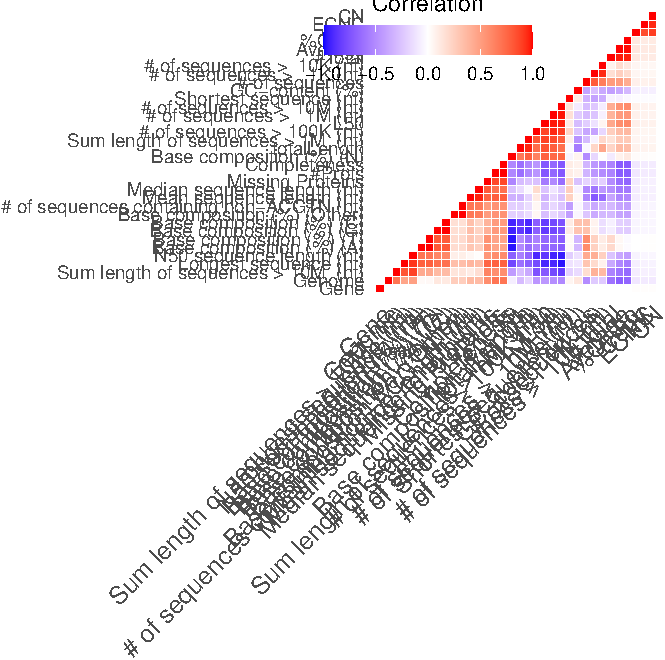
\includegraphics{paper_PLOS_draft_files/figure-latex/Correlations between genome quality scores-1.pdf}

\begin{verbatim}
## Warning: Column `Genome`/`BestGenome` joining factor and character vector,
## coercing into character vector
\end{verbatim}

\begin{verbatim}
## Warning: `as.tibble()` is deprecated as of tibble 2.0.0.
## Please use `as_tibble()` instead.
## The signature and semantics have changed, see `?as_tibble`.
## This warning is displayed once every 8 hours.
## Call `lifecycle::last_warnings()` to see where this warning was generated.
\end{verbatim}

\begin{verbatim}
## Warning: Removed 1 rows containing missing values (geom_text).
\end{verbatim}

\begin{figure}
\centering
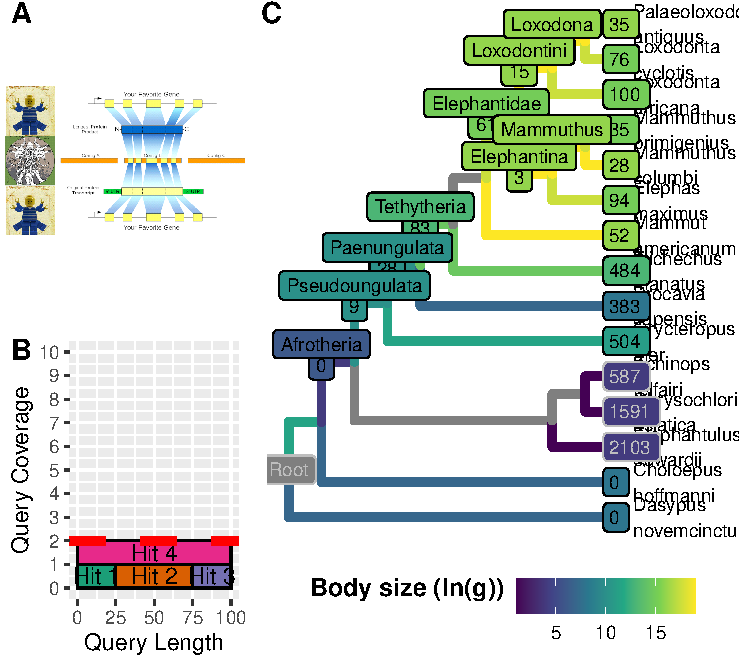
\includegraphics{paper_PLOS_draft_files/figure-latex/Figure 2-1.pdf}
\caption{Figure 2: A Reciprocal Best-Hit BLAT pipeline for identifying
gene copy number in other genomes. A) A graphic summary of the
reciprocal best-hit strategy. B) Estimated Copy Number by Coverage. C)}
\end{figure}

\begin{verbatim}
## Warning: Table 2
\end{verbatim}

Enhanced cancer suppression may have evolved through many mechanisms;
among the most parsimonious is an increase in the copy number of genes
with tumor suppressor functions. Previous studies focusing on candidate
gene studies, for example, have identified increased copy number of the
tumor suppressors \emph{TP53} and \emph{LIF} in elephants
{[}{\textbf{???}},11,21--23{]}. Therefore, in order to test whether this
was a pervasive phenomena genome-wide in \emph{Afrotherians}, we used a
Reciprocal Best Hit BLAT (RBHB) approach to infer gene copy number in
\emph{Afrotherian} and \emph{Atlantogenatan} genomes (Fig. 2A). Because
RBHB-like approaches can over-estimate copy number when genes are
fragmented or incorrectly assembled across multiple scaffolds, we also
inferred copy number using a complementary method that quantifies the
ratio between observed and expected gene coverage per nucleotide (ECNC)
(Fig. 2B; Sup. Fig. 2A-D). By only including nucleotides from the query
sequence that were observed in the target genome, we also correct for
partial hits where some or all of the homologs of a gene have diverged
from the human homolog.

Because our sequence database included various protein transcripts for
each gene, in order to obtain gene-level copy number information and
elimate any many-to-one mappings of hits, we labeled each exon of every
reciprocal best hit (RBH) with the gene corresponding to the query
transcript and merged all overlapping exons; next, we eliminated any
many-to-one exons that resulted from the previous step. Finally, we
reassembled the gene loci based on the original transcript starts and
ends, and the collapsed exon data, obtaining the full sequence of each
RBH locus. Genes were considered to be duplicated if its copy number via
RBHB was greater than or equal to 2, and the maximum ECNC among all
transcripts prior to filtering was greater than or equal to 1.50. This
cutoff of ECNC was selected to account for truncated gene duplications,
which have been shown to be functional in various examples
{[}{\textbf{???}} examples of this{]}.

To reconcile the Atlantogenatan phylogeny with duplication events, we
used maximum likelihood to reconstruct likely ancestral copy numbers for
each gene at each node in the phylogeny. To define the copy number of a
gene, we conservatively used the lesser value between the RBHB hit
count, and the ECNC value rounded to the nearest whole number. In order
to perform

Next, in order to select genes and duplicates which were likely
functional, we omitted any hits that were not supported by either the
gene prediction method GenScan, or by at least one transcript assembled
from publically-available RNA-seq data.

We describe the number of genes that increased in each lineage in
\emph{Atlantogenata} in Figure 2. Among the genes that increased in copy
number in the elephant lineage are TP53 and LIF, as previously
described. Furthermore, we identify

\hypertarget{duplications-that-occured-recently-in-probodiscea-are-enriched-for-tumor-suppressor-pathways}{%
\subsection{Duplications that occured recently in Probodiscea are
enriched for tumor suppressor
pathways}\label{duplications-that-occured-recently-in-probodiscea-are-enriched-for-tumor-suppressor-pathways}}

In order to infer the functional consequences of these gene
duplications, we tested if duplicate genes were enriched in specific
pathways relative to our initial query set of genes. We used

\hypertarget{retroduplication-of-eef1a1-in-the-stem-lineage-of-tehthytheria}{%
\subsection{Retroduplication of EEF1A1 in the stem-lineage of
Tehthytheria}\label{retroduplication-of-eef1a1-in-the-stem-lineage-of-tehthytheria}}

\begin{verbatim}
## Warning: Fig 3: EEF1A1
\end{verbatim}

Previous studies have identified genes whose transgenic overexpression
delays aging related phenotypes and extends lifespan. Overexpression of
the eukaryotic translation elongation factor 1 alpha 1 (EEF1A1) gene,
for example, extends lifespan in transgenic Drosophila. Like most
mammalian genomes, we found that Afrotherian genomes encoded numerous
EEF1A1 retrogenes (Fig. XA). While the majority of these retrogenes have
premature stop codons and insertions/deletions characteristic of
pseudogenes, at least 13 Tehthytherian-specific EEF1A1 retrogenes have
the potential to encode functional proteins (Fig. XB). Unfortunately it
is difficult to determine if these retrogenes are transcribed because
they have relatively high sequence similarity (83-88\%), suggesting
evidence of transcription using RNA-Seq data is likely an artifact.
Indeed, nearly all of the EEF1A1 retrogene transcripts assembled by
StringTie were confined to their gene body and UTRs and thus lacked
unique sequences. The EEF1A1RTG13 transcript, however, initiates within
an upstream MLT1B retrovirus-like MaLR transposable element and includes
unique 5?- and 3?-UTR sequences, indicating at least one EEF1A1
retrogene is transcribed (Fig. XC). EEF1A1

Candidate gene studies, for example, have identified functional
duplicates of the tumor suppressors TP53 and LIF in elephants. In a
larger candidate gene study, Caulin et al.~characterized the copy number
of 830 known tumor-suppressor genes across 36 mammals and identified 382
putative duplicates, including duplicates in species with large body
sizes and long life-spans. however, the probability of developing cancer
is similar for small, short-lived mammals such as mice and for large,
long-lived mammals such as elephants.

In stark contrast, genome-wide studies of unusually large or long-lived
species such as the bowhead whale (Keane et al., 2015), Myotid bats
(Seim et al., 2013; Zhang et al., 2013), naked mole rat (Kim et al.,
2011), and blind mole rat (Fang et al., 2014) did not find an over
representation of tumor suppressors among duplicate genes.

A genomic analysis of genetic changes associated with the evolution of
enhanced cancer resistance in the elephant lineage has yet to be
performed. Thus it is not clear if the duplication of TP53 and LIF
reflects a general pattern of tumor suppressor duplication in the
elephant lineage, unlike other lineages that resolved Peto?s paradox, or
from the kinds of ascertainment biases common in candidate gene studies.

\hypertarget{concerted-duplication-of-tp53-and-tp53-related-genes-towards-probodiscea}{%
\subsection{\texorpdfstring{Concerted duplication of TP53 and
TP53-related genes towards
\emph{Probodiscea}}{Concerted duplication of TP53 and TP53-related genes towards Probodiscea}}\label{concerted-duplication-of-tp53-and-tp53-related-genes-towards-probodiscea}}

\begin{verbatim}
## Warning: Fig4
\end{verbatim}

\hypertarget{step-wise-reduction-of-intrinsic-cancer-risk-in-large-long-lived-afrotherians}{%
\subsection{Step-wise reduction of intrinsic cancer risk in large,
long-lived
Afrotherians}\label{step-wise-reduction-of-intrinsic-cancer-risk-in-large-long-lived-afrotherians}}

\begin{verbatim}
## # A tibble: 253 x 6
##     parent  node branch.length label                       lnSize Lifespan
##      <int> <int>         <dbl> <chr>                        <dbl>    <dbl>
##   1    135     1     40.1      Geogale.aurita                   2    1.72 
##   2    140     2    122.       Limnogale.mergulus               5    2.30 
##   3    140     3      0.135    Microgale.taiva                  2    1.72 
##   4    139     4     33.5      Microgale.parvula                1    1.52 
##   5    138     5      0.595    Microgale.brevicaudata           2    1.72 
##   6    142     6      0.571    Microgale.cowani                 3    1.91 
##   7    142     7      1.07     Microgale.jobihely               2    1.72 
##   8    145     8      0.772    Microgale.longicaudata           2    1.72 
##   9    145     9      0.173    Microgale.principula             2    1.72 
##  10    144    10     34.3      Microgale.pusilla                1    1.52 
##  11    143    11     61.4      Microgale.talazaci               4    1.76 
##  12    136    12     22.8      Oryzorictes.hova                 4    2.11 
##  13    147    13      7.75     Echinops.telfairi                4    2.94 
##  14    147    14     12.5      Setifer.setosus                  6    2.65 
##  15    148    15      4.68     Hemicentetes.semispinosus        5    0.993
##  16    148    16     79.5      Tenrec.ecaudatus                 7    2.16 
##  17    150    17      2.82     Micropotamogale.lamottei         4    2.11 
##  18    150    18    103.       Potamogale.velox                 6    2.50 
##  19    151    19     69.8      Protenrec.tricuspis              1    1.52 
##  20    151    20      2.21     Dilambdogale.gheerbranti         2    1.72 
##  21    157    21      0.454    Carpitalpa.arendsi               4    2.11 
##  22    158    22      3.26     Neamblysomus.gunningi            4    2.11 
##  23    158    23      5.72     Neamblysomus.julianae            3    1.91 
##  24    162    24      0.976    Amblysomus.corriae               4    2.11 
##  25    162    25      1.38     Amblysomus.robustus              4    2.11 
##  26    161    26      0.524    Amblysomus.septentrionalis       4    2.11 
##  27    160    27      0.0152   Amblysomus.hottentotus           4    2.11 
##  28    159    28      3.79     Amblysomus.marleyi               4    2.11 
##  29    163    29      0.321    Chlorotalpa.duthieae             3    1.91 
##  30    163    30      0.0874   Chlorotalpa.sclateri             4    2.11 
##  31    165    31     62.8      Chrysospalax.trevelyani          6    2.50 
##  32    165    32      0.130    Chrysospalax.villosus            5    2.30 
##  33    164    33     13.4      Calcochloris.obtusirostris       3    1.91 
##  34    153    34      9.65     Eremitalpa.granti                3    1.91 
##  35    167    35      3.34     Chrysochloris.asiatica           4    2.11 
##  36    167    36      5.78     Cryptochloris.wintoni            3    1.91 
##  37    166    37      0.333    Chrysochloris.stuhlmanni         4    2.11 
##  38    175    38      0.926    Elephantulus.brachyrhynchus      4    2.11 
##  39    175    39      0.118    Elephantulus.rufescens           4    2.07 
##  40    176    40      1.15     Elephantulus.intufi              4    2.23 
##  41    176    41      0.319    Elephantulus.rupestris           4    2.11 
##  42    177    42      0.237    Elephantulus.edwardii            4    2.11 
##  43    177    43      0.953    Elephantulus.myurus              4    2.11 
##  44    179    44     10.5      Elephantulus.rozeti              4    1.97 
##  45    179    45     24.6      Petrodromus.tetradactylus        5    2.30 
##  46    178    46     14.2      Macroscelides.proboscideus       4    2.16 
##  47    181    47      1.93     Elephantulus.fuscipes            4    2.11 
##  48    182    48      0.678    Elephantulus.fuscus              4    2.11 
##  49    182    49      1.10     Elephantulus.revoili             3    1.91 
##  50    184    50      0.403    Rhynchocyon.chrysopygus          6    2.40 
##  51    185    51      3.30     Rhynchocyon.cirnei               6    2.50 
##  52    185    52      4.33     Rhynchocyon.udzungwensis         7    2.69 
##  53    183    53      2.13     Rhynchocyon.petersi              6    2.50 
##  54    170    54     15.9      Metoldobotes.sp..nov             6    2.50 
##  55    186    55     11.8      Chambius.kasserinensis           4    2.11 
##  56    186    56     11.6      Herodotius.pattersoni            5    2.30 
##  57    188    57      6.59     Orycteropus.afer                11    3.39 
##  58    188    58      0.569    Myorycteropus.africanus         10    3.27 
##  59    194    59      1.86     Dendrohyrax.dorsalis             8    2.88 
##  60    195    60      1.64     Heterohyrax.brucei               8    2.88 
##  61    195    61      0.000068 Procavia.capensis                8    2.69 
##  62    193    62      1.15     Thyrohyrax.domorictus            9    3.08 
##  63    192    63      3.55     Thyrohyrax.meyeri                9    3.08 
##  64    198    64     28.6      Thyrohyrax.litholagus           10    3.27 
##  65    201    65      2.29     Pachyhyrax.crassidentatus       12    3.66 
##  66    201    66      1.45     Bunohyrax.fajumensis            11    3.47 
##  67    202    67      5.44     Geniohyus.mirus                 11    3.47 
##  68    202    68     11.4      Bunohyrax.major                 12    3.66 
##  69    203    69      0.235    Megalohyrax.eocaenus            12    3.66 
##  70    203    70      7.21     Megalohyrax.sp..nov             13    3.86 
##  71    207    71      0.0699   Titanohyrax.andrewsi            13    3.86 
##  72    207    72     34.6      Titanohyrax.ultimus             14    4.05 
##  73    206    73      0.0353   Titanohyrax.angustidens         12    3.66 
##  74    205    74     13.7      Antilohyrax.pectidens           11    3.47 
##  75    204    75      0.194    Afrohyrax.championi             11    3.47 
##  76    209    76      2.90     Saghatherium.antiquum           10    3.27 
##  77    209    77     15.0      Selenohyrax.chatrathi           11    3.47 
##  78    208    78     15.8      Saghatherium.bowni               9    3.08 
##  79    211    79      2.82     Seggeurius.amourensis            8    2.88 
##  80    211    80      0.733    Microhyrax.lavocati              8    2.88 
##  81    210    81     18.2      Dimaitherium.patnaiki           10    3.27 
##  82    220    82      5.81     Elephas.maximus                 15    4.18 
##  83    222    83      6.12     Elephas.antiquus.falconeri      12    3.66 
##  84    222    84      1.90     Elephas.cypriotes               12    3.66 
##  85    221    85      0.340    Elephas.maximus.asurus          16    4.44 
##  86    223    86     16.0      Mammuthus.trogontherii          16    4.44 
##  87    224    87      0.910    Mammuthus.columbi               16    4.44 
##  88    224    88      2.17     Mammuthus.primigenius           15    4.24 
##  89    225    89      1.28     Loxodonta.africana              15    4.17 
##  90    227    90      0.0149   Palaeoloxodon.antiquus          16    4.44 
##  91    227    91     12.8      Palaeoloxodon.namadicus         17    4.63 
##  92    226    92      3.72     Loxodonta.cyclotis              15    4.24 
##  93    228    93     15.3      Mammut.borsoni                  16    4.44 
##  94    228    94      0.951    Mammut.americanum               16    4.44 
##  95    216    95      3.64     Phiomia.spp                     14    4.05 
##  96    230    96      0.0280   Omanitherium.dhofarensis        13    3.86 
##  97    230    97      7.29     Arcanotherium.savagei           13    3.86 
##  98    229    98     73.6      Barytherium.spp                 15    4.24 
##  99    214    99      5.71     Moeritherium.spp                14    4.05 
## 100    231   100    326.       Phosphatherium.escuilliei       10    3.27 
## 101    232   101      2.29     Numidotherium.koholense         13    3.86 
## 102    232   102      0.742    Daouitherium.rebouli            13    3.86 
## 103    235   103      5.85     Dugong.dugon                    13    4.29 
## 104    235   104    173.       Hydrodamalis.gigas              16    4.44 
## 105    237   105      0.688    Trichechus.inunguis             13    3.69 
## 106    237   106      1.39     Trichechus.manatus              13    4.23 
## 107    236   107      0.574    Trichechus.senegalensis         13    3.86 
## 108    238   108     13.6      Prorastomus.sirenoides          11    3.47 
## 109    238   109     33.7      Protosiren.smithae              13    3.86 
## 110    241   110      0.640    Choloepus.didactylus             9    3.61 
## 111    241   111      0.316    Choloepus.hoffmanni              8    3.71 
## 112    242   112      0.0297   Bradypus.torquatus               8    2.88 
## 113    243   113      0.483    Bradypus.tridactylus             8    2.88 
## 114    243   114      0.512    Bradypus.variegatus              8    2.88 
## 115    245   115     10.4      Tamandua.tetradactyla            9    2.94 
## 116    245   116     41.0      Myrmecophaga.tridactyla         10    3.43 
## 117    244   117      2.15     Cyclopes.didactylus              9    3.08 
## 118    249   118     15.0      Euphractus.sexcinctus            8    3.10 
## 119    249   119      5.54     Zaedyus.pichiy                   7    2.53 
## 120    250   120      0.0899   Chaetophractus.nationi           8    2.88 
## 121    250   121      0.418    Chaetophractus.villosus          8    3.23 
## 122    251   122    268.       Priodontes.maximus              11    2.71 
## 123    252   123     16.0      Tolypeutes.matacus               7    3.61 
## 124    252   124      0.248    Cabassous.centralis              8    2.88 
## 125    253   125      4.05     Dasypus.hybridus                 7    2.69 
## 126    253   126     74.1      Dasypus.kappleri                 9    3.08 
## 127    253   127     14.7      Dasypus.novemcinctus             8    3.10 
## 128    253   128     12.2      Dasypus.sabanicola               7    2.69 
## 129    253   129      4.44     Dasypus.septemcinctus            7    2.82 
## 130    130   130     NA        Atlantogenata                    2    1.72 
## 131    130   131      0.000982 Afrotheria                       6    2.50 
## 132    131   132     44.5      Afrosorcida                      4    2.11 
## 133    132   133     11.8      <NA>                             4    2.11 
## 134    133   134      0.420    <NA>                             4    2.11 
## 135    134   135     10.1      <NA>                             3    1.91 
## 136    135   136      0.373    <NA>                             3    1.91 
## 137    136   137      2.96     <NA>                             3    1.91 
## 138    137   138      2.69     <NA>                             3    1.91 
## 139    138   139      0.450    <NA>                             2    1.72 
## 140    139   140      3.36     <NA>                             3    1.91 
## 141    137   141      0.153    <NA>                             3    1.91 
## 142    141   142      0.116    <NA>                             2    1.72 
## 143    141   143      0.222    <NA>                             2    1.72 
## 144    143   144      0.771    <NA>                             2    1.72 
## 145    144   145      0.109    <NA>                             3    1.91 
## 146    134   146     38.5      <NA>                             5    2.30 
## 147    146   147      1.81     <NA>                             3    1.91 
## 148    146   148      5.26     <NA>                             3    1.91 
## 149    133   149      4.28     <NA>                             3    1.91 
## 150    149   150     52.3      <NA>                             5    2.30 
## 151    149   151     15.6      <NA>                             3    1.91 
## 152    132   152     12.0      <NA>                             4    2.11 
## 153    152   153      0.0295   <NA>                             4    2.11 
## 154    153   154      0.173    <NA>                             3    1.91 
## 155    154   155      0.0141   <NA>                             3    1.91 
## 156    155   156      0.107    <NA>                             4    2.11 
## 157    156   157      0.00544  <NA>                             3    1.91 
## 158    157   158      0.102    <NA>                             3    1.91 
## 159    156   159      0.150    <NA>                             3    1.91 
## 160    159   160      0.483    <NA>                             3    1.91 
## 161    160   161      0.321    <NA>                             3    1.91 
## 162    161   162      0.00743  <NA>                             4    2.11 
## 163    155   163      2.12     <NA>                             3    1.91 
## 164    154   164      0.774    <NA>                             4    2.11 
## 165    164   165     18.6      <NA>                             5    2.30 
## 166    152   166      0.260    <NA>                             3    1.91 
## 167    166   167      0.155    <NA>                             3    1.91 
## 168    131   168      0.00016  <NA>                             6    2.50 
## 169    168   169      2.49     Macroscelidae                    5    2.30 
## 170    169   170      0.105    <NA>                             5    2.30 
## 171    170   171      4.23     <NA>                             5    2.30 
## 172    171   172      6.20     <NA>                             3    1.91 
## 173    172   173      0.977    <NA>                             3    1.91 
## 174    173   174      0.448    <NA>                             4    2.11 
## 175    174   175      0.349    <NA>                             4    2.11 
## 176    174   176      0.176    <NA>                             4    2.11 
## 177    173   177      1.62     <NA>                             4    2.11 
## 178    172   178      0.155    <NA>                             3    1.91 
## 179    178   179      0.180    <NA>                             4    2.11 
## 180    171   180      0.100    <NA>                             5    2.30 
## 181    180   181     11.2      <NA>                             3    1.91 
## 182    181   182     12.0      <NA>                             3    1.91 
## 183    180   183     30.6      <NA>                             3    1.91 
## 184    183   184      2.34     <NA>                             3    1.91 
## 185    184   185      0.0165   <NA>                             3    1.91 
## 186    169   186      4.53     <NA>                             5    2.30 
## 187    168   187    546.       Pseudoungulata                  10    3.27 
## 188    187   188     12.9      <NA>                            10    3.27 
## 189    187   189      4.42     Paenungulata                    10    3.27 
## 190    189   190      6.90     <NA>                             5    2.30 
## 191    190   191      1.47     <NA>                            10    3.27 
## 192    191   192     17.9      <NA>                             9    3.08 
## 193    192   193      0.00758  <NA>                             9    3.08 
## 194    193   194     19.5      <NA>                             5    2.30 
## 195    194   195      2.67     <NA>                             5    2.30 
## 196    191   196      5.61     <NA>                             3    1.91 
## 197    196   197      8.46     <NA>                             3    1.91 
## 198    197   198      0.602    <NA>                            11    3.47 
## 199    198   199      8.81     <NA>                            12    3.66 
## 200    199   200      0.347    <NA>                             3    1.91 
## 201    200   201      0.177    <NA>                            12    3.66 
## 202    200   202      0.584    <NA>                             3    1.91 
## 203    199   203      8.90     <NA>                            12    3.66 
## 204    197   204      9.93     <NA>                            11    3.47 
## 205    204   205      1.23     <NA>                            12    3.66 
## 206    205   206     22.2      <NA>                             3    1.91 
## 207    206   207     10.2      <NA>                            13    3.86 
## 208    196   208      6.63     <NA>                             3    1.91 
## 209    208   209      1.16     <NA>                            10    3.27 
## 210    190   210     22.7      <NA>                             9    3.08 
## 211    210   211      8.32     <NA>                             8    2.88 
## 212    189   212    187.       Tethytheria                     13    3.86 
## 213    212   213      3.40     <NA>                             3    1.91 
## 214    213   214      6.37     <NA>                            13    3.86 
## 215    214   215      1.15     <NA>                            14    4.05 
## 216    215   216     13.4      <NA>                             3    1.91 
## 217    216   217     30.3      Proboscidae                      3    1.91 
## 218    217   218      2.21     Elephantidae                    15    4.24 
## 219    218   219      0.0116   Elephantina                     16    4.44 
## 220    219   220      0.128    <NA>                            15    4.24 
## 221    220   221      0.369    <NA>                             3    1.91 
## 222    221   222    400.       <NA>                             3    1.91 
## 223    219   223      0.645    <NA>                             3    1.91 
## 224    223   224      0.467    Mammuthus                       16    4.44 
## 225    218   225      0.108    Loxodontini                     16    4.44 
## 226    225   226      0.862    Loxodona                        16    4.44 
## 227    226   227      6.09     <NA>                             3    1.91 
## 228    217   228      9.63     <NA>                             3    1.91 
## 229    215   229      0.197    <NA>                             3    1.91 
## 230    229   230      2.47     <NA>                             3    1.91 
## 231    213   231      0.128    <NA>                            13    3.86 
## 232    231   232      0.268    <NA>                             3    1.91 
## 233    212   233      0.309    <NA>                            12    3.66 
## 234    233   234     16.4      <NA>                             3    1.91 
## 235    234   235      0.530    <NA>                             3    1.91 
## 236    234   236      0.134    <NA>                             3    1.91 
## 237    236   237      0.145    <NA>                             3    1.91 
## 238    233   238      3.59     <NA>                             3    1.91 
## 239    130   239    125.       Xenarthra                       11    3.47 
## 240    239   240     14.6      <NA>                             3    1.91 
## 241    240   241      3.04     <NA>                             3    1.91 
## 242    240   242      0.0660   <NA>                            11    3.47 
## 243    242   243      0.112    <NA>                            11    3.47 
## 244    239   244     15.1      <NA>                             3    1.91 
## 245    244   245     21.7      <NA>                             9    3.08 
## 246    239   246      0.958    <NA>                            10    3.27 
## 247    246   247      0.0602   <NA>                             3    1.91 
## 248    247   248      0.0914   <NA>                             3    1.91 
## 249    248   249      0.000579 <NA>                             8    2.88 
## 250    248   250      0.000908 <NA>                            11    3.47 
## 251    247   251      0.217    <NA>                             3    1.91 
## 252    251   252      0.0523   <NA>                            11    3.47 
## 253    246   253      0.140    <NA>                             8    2.88
\end{verbatim}

\begin{verbatim}
## Warning: Fig5
\end{verbatim}

The dramatic increase in body mass and lifespan in some Afrotherian
lineages implies those lineages evolved reduced cancer risk. To infer
the magnitude of these reductions we estimated differences in cancer
risk between small bodied, short-lived species and large bodied,
long-lived species as well as for reconstructed ancestral Afrotherians.
Following {[}{\textbf{???}}{]} we estimate the intrinsic cancer risk as
the product of risk associated with body mass and lifespan. Differences
in cancer susceptibility due to body mass differences between species
can be approximated simply as the fold difference in body mass (\(D\))
between species {[}{\textbf{???}}{]}. The risk of developing cancer also
increases in proportion to the sixth power of age and is approximated by
the formula \(Ct^6\), in which the proportionality constant C that
determines susceptibility to cancer induction is multiplied by the sixth
power of the age in years, \(t\)
{[}{\textbf{???}},{\textbf{??}},{\textbf{??}}{]}. Thus we can estimate
differences in the intrinsic cancer risk between species as \(D(Ct^6)\).
We inferred that susceptibility to cancer induction (\(C\)) was reduced
3.40x10\^{}3-fold in the ancestor of Pseudoungulata, 7.20×10\^{}3-fold
in the ancestor of Paenungulata, 8.81x10\^{}5-fold in the ancestor of
Tehthytheria, 1.46x10\^{}8-fold in the ancestor of Proboscidea, and
1.28x10\^{}6-fold in the ancestor of Sirenia relative to the ancestral
Afrotherian (Table 3). What biological mechanisms underlie the evolution
of thousand- to hundred million-fold reductions in cancer susceptibility
during the origins of Afrotherians, which are essential for large body
size and long lifespan to evolve

\hypertarget{other-figures}{%
\section{OTHER FIGURES}\label{other-figures}}

\hypertarget{references}{%
\section*{References}\label{references}}
\addcontentsline{toc}{section}{References}

\hypertarget{refs}{}
\leavevmode\hypertarget{ref-Green2011}{}%
1. Green J, Cairns BJ, Casabonne D, Wright FL, Reeves G, Beral V, et al.
Height and cancer incidence in the Million Women Study: prospective
cohort, and meta-analysis of prospective studies of height and total
cancer risk. The Lancet Oncology. 2011;12: 785--794.
doi:\href{https://doi.org/10.1016/s1470-2045(11)70154-1}{10.1016/s1470-2045(11)70154-1}

\leavevmode\hypertarget{ref-Nunney:20181c2}{}%
2. Nunney L. Size matters: height, cell number and a person's risk of
cancer. Proc R Soc B. 2018;285: 20181743.
doi:\href{https://doi.org/10.1098/rspb.2018.1743}{10.1098/rspb.2018.1743}

\leavevmode\hypertarget{ref-Dobson2013}{}%
3. Dobson JM. Breed-predispositions to cancer in pedigree dogs. ISRN
veterinary science. 2013;2013: 941275.
doi:\href{https://doi.org/10.1155/2013/941275}{10.1155/2013/941275}

\leavevmode\hypertarget{ref-CaulinAndMaley2011}{}%
4. Caulin AF, Maley CC. Peto's Paradox: evolution's prescription for
cancer prevention. Trends in ecology \& evolution. 2011;26: 175--82.
doi:\href{https://doi.org/10.1016/j.tree.2011.01.002}{10.1016/j.tree.2011.01.002}

\leavevmode\hypertarget{ref-Leroi2003}{}%
5. Leroi AM, Koufopanou V, Burt A. Cancer selection. Nature Reviews
Cancer. 2003;3: 226--231.
doi:\href{https://doi.org/10.1038/nrc1016}{10.1038/nrc1016}

\leavevmode\hypertarget{ref-Peto1975}{}%
6. Peto R, Roe F, Lee P, Levy L, Clack J. Cancer and ageing in mice and
men. British Journal of Cancer. 1975;32: 411--426.
doi:\href{https://doi.org/10.1038/bjc.1975.242}{10.1038/bjc.1975.242}

\leavevmode\hypertarget{ref-Ashur-Fabian2004}{}%
7. Ashur-Fabian O, Avivi A, Trakhtenbrot L, Adamsky K, Cohen M, Kajakaro
G, et al. Evolution of p53 in hypoxia-stressed Spalax mimics human tumor
mutation. Proceedings of the National Academy of Sciences. 2004;101:
12236--12241.
doi:\href{https://doi.org/10.1073/pnas.0404998101}{10.1073/pnas.0404998101}

\leavevmode\hypertarget{ref-Seluanov2008}{}%
8. Seluanov A, Hine C, Bozzella M, Hall A, Sasahara THC, Ribeiro AACM,
et al. Distinct tumor suppressor mechanisms evolve in rodent species
that differ in size and lifespan. Aging cell. 2008;7: 813--23.
doi:\href{https://doi.org/10.1111/j.1474-9726.2008.00431.x}{10.1111/j.1474-9726.2008.00431.x}

\leavevmode\hypertarget{ref-Gorbunova2012}{}%
9. Gorbunova V, Hine C, Tian X, Ablaeva J, Gudkov AV, Nevo E, et al.
Cancer resistance in the blind mole rat is mediated by concerted
necrotic cell death mechanism. Proceedings of the National Academy of
Sciences of the United States of America. 2012;109: 19392--6.
doi:\href{https://doi.org/10.1073/pnas.1217211109}{10.1073/pnas.1217211109}

\leavevmode\hypertarget{ref-Tian2013}{}%
10. Tian X, Azpurua J, Hine C, Vaidya A, Myakishev-Rempel M, Ablaeva J,
et al. High molecular weight hyaluronan mediates the cancer resistance
of the naked mole-rat. 2013;499.
doi:\href{https://doi.org/10.1038/nature12234}{10.1038/nature12234}

\leavevmode\hypertarget{ref-Sulak2016}{}%
11. Sulak M, Fong L, Mika K, Chigurupati S, Yon L, Mongan NP, et al.
TP53 copy number expansion is associated with the evolution of increased
body size and an enhanced DNA damage response in elephants. eLife.
2016;5: e11994.
doi:\href{https://doi.org/10.7554/elife.11994}{10.7554/elife.11994}

\leavevmode\hypertarget{ref-HAGR}{}%
12. Tacutu R, Craig T, Budovsky A, Wuttke D, Lehmann G, Taranukha D, et
al. Human Ageing Genomic Resources: Integrated databases and tools for
the biology and genetics of ageing. Nucleic Acids Research. 2013;41:
D1027--D1033.
doi:\href{https://doi.org/10.1093/nar/gks1155}{10.1093/nar/gks1155}

\leavevmode\hypertarget{ref-Schwartz1995}{}%
13. Schwartz GT, Rasmussen DT, Smith RJ. Body-Size Diversity and
Community Structure of Fossil Hyracoids. Journal of Mammalogy. 1995;76:
1088--1099. doi:\href{https://doi.org/10.2307/1382601}{10.2307/1382601}

\leavevmode\hypertarget{ref-Scheffer1972}{}%
14. Scheffer VB. The Weight of the Steller Sea Cow. Journal of
Mammalogy. 1972;53: 912--914.
doi:\href{https://doi.org/10.2307/1379236}{10.2307/1379236}

\leavevmode\hypertarget{ref-Larramendi:20151c2}{}%
15. Larramendi A. Shoulder Height, Body Mass, and Shape of
Proboscideans. Acta Palaeontologica Polonica. 2015;61.
doi:\href{https://doi.org/10.4202/app.00136.2014}{10.4202/app.00136.2014}

\leavevmode\hypertarget{ref-OLeary2013a}{}%
16. O'Leary MA, Bloch JI, Flynn JJ, Gaudin TJ, Giallombardo A, Giannini
NP, et al. The placental mammal ancestor and the post-K-Pg radiation of
placentals. Science (New York, NY). 2013;339: 662--7.
doi:\href{https://doi.org/10.1126/science.1229237}{10.1126/science.1229237}

\leavevmode\hypertarget{ref-Springer2013}{}%
17. Springer MS, Meredith RW, Teeling EC, Murphy WJ. Technical comment
on "The placental mammal ancestor and the post-K-Pg radiation of
placentals". Science (New York, NY). 2013;341: 613.
doi:\href{https://doi.org/10.1126/science.1238025}{10.1126/science.1238025}

\leavevmode\hypertarget{ref-OLeary2013b}{}%
18. O'Leary MA, Bloch JI, Flynn JJ, Gaudin TJ, Giallombardo A, Giannini
NP, et al. Response to comment on "The placental mammal ancestor and the
post-K-Pg radiation of placentals". Science (New York, NY). 2013;341:
613.
doi:\href{https://doi.org/10.1126/science.1238162}{10.1126/science.1238162}

\leavevmode\hypertarget{ref-PuttickAndThomas2015}{}%
19. Puttick MN, Thomas GH. Fossils and living taxa agree on patterns of
body mass evolution: a case study with Afrotheria. Proceedings
Biological sciences / The Royal Society. 2015;282: 20152023.
doi:\href{https://doi.org/10.1098/rspb.2015.2023}{10.1098/rspb.2015.2023}

\leavevmode\hypertarget{ref-Abegglen:JAMA2015}{}%
20. Abegglen LM, Caulin AF, Chan A, Lee K, Robinson R, Campbell MS, et
al. Potential Mechanisms for Cancer Resistance in Elephants and
Comparative Cellular Response to DNA Damage in Humans. JAMA. 2015;314:
1850--1860.
doi:\href{https://doi.org/10.1001/jama.2015.13134}{10.1001/jama.2015.13134}

\leavevmode\hypertarget{ref-Vazquez2018}{}%
21. Vazquez JM, Sulak M, Chigurupati S, Lynch VJ. A Zombie LIF Gene in
Elephants Is Upregulated by TP53 to Induce Apoptosis in Response to DNA
Damage. Cell Reports. 2018;24: 1765--1776.
doi:\href{https://doi.org/10.1016/j.celrep.2018.07.042}{10.1016/j.celrep.2018.07.042}

\leavevmode\hypertarget{ref-Caulin2015}{}%
22. Caulin AF, Graham TA, Wang L-S, Maley CC. Solutions to Peto's
paradox revealed by mathematical modelling and cross-species cancer gene
analysis. Philosophical transactions of the Royal Society of London
Series B, Biological sciences. 2015;370: 20140222.
doi:\href{https://doi.org/10.1098/rstb.2014.0222}{10.1098/rstb.2014.0222}

\leavevmode\hypertarget{ref-Doherty2016}{}%
23. Doherty A, Magalhães J de. Has gene duplication impacted the
evolution of Eutherian longevity? Aging Cell. 2016;15: 978--980.
doi:\href{https://doi.org/10.1111/acel.12503}{10.1111/acel.12503}

\leavevmode\hypertarget{ref-Bininda-Emonds2008}{}%
24. Bininda-Emonds ORP, Cardillo M, Jones KE, MacPhee RDE, Beck RMD,
Grenyer R, et al. Erratum: The delayed rise of present-day mammals.
Nature. 2008;456: 274--274.
doi:\href{https://doi.org/10.1038/nature07347}{10.1038/nature07347}

\leavevmode\hypertarget{ref-ElliotAndMooers2014}{}%
25. Elliot MG, Mooers AØ. Inferring ancestral states without assuming
neutrality or gradualism using a stable model of continuous character
evolution. BMC evolutionary biology. 2014;14: 226.
doi:\href{https://doi.org/10.1186/s12862-014-0226-8}{10.1186/s12862-014-0226-8}

\leavevmode\hypertarget{ref-blat}{}%
26. Kent JW. BLAT---The BLAST-Like Alignment Tool. Genome Research.
2002;12: 656--664.
doi:\href{https://doi.org/10.1101/gr.229202}{10.1101/gr.229202}

\leavevmode\hypertarget{ref-AltenhoffAndDessimoz2009}{}%
27. Altenhoff AM, Dessimoz C. Phylogenetic and functional assessment of
orthologs inference projects and methods. PLoS computational biology.
2009;5: e1000262.
doi:\href{https://doi.org/10.1371/journal.pcbi.1000262}{10.1371/journal.pcbi.1000262}

\leavevmode\hypertarget{ref-uniprot}{}%
28. Consortium TU. UniProt: the universal protein knowledgebase. Nucleic
Acids Research. 2017;45: D158--D169.
doi:\href{https://doi.org/10.1093/nar/gkw1099}{10.1093/nar/gkw1099}

\nolinenumbers


\end{document}

